% Archivo generado automáticamente con los problemas
\section*{Problems}
Sección: 8_Spin_1_and_gauge_invariance
Páginas: 157-158
Contenido:
8.7.3 Spin greater than 2
One can continue this procedure for integer spin greater than 2. There exist spin-3 particles
in nature, for example the ω3 with mass of 1670 MeV, as well as spin 4, spin 5, etc. These
particles are all massive. One can construct free Lagrangians for them using the same trick.
An interesting and profound result is that it is impossible to have an interacting theory of
massless particles with spin greater than 2. The required gauge invariance would be so
restrictive that nothing could satisfy it. We will prove this in the next chapter. Constructing
the kinetic term for a spin-3 particle is done in Problem 8.8.
Problems

8.1 Show that having a probability interpretation, with 0 ≤P ≤1, requires us to have
only positive (or only negative) norm states.

8.2 Calculate the energy-momentum tensor corresponding to the Lagrangian L =
−1
4F 2
μν. Show that the energy density is positive definite, up to a total spatial
derivative E −∂iX > 0.

8.3 Calculate the classical propagator for a massive spin-1 particle by inverting the
equations of motion to the form Aμ = ΠμνJν.

8.4 Calculate the Feynman propagator for a photon. Show that Eq. (8.102) is correct.

8.5 Vector polarization sums. In this problem you can build some intuition for the way
in which the numerator of a spin-1 particle propagator represents an outer product
of physical polarizations |ϵ⟩⟨ϵ|. Calculate the 4 × 4 matrix outer product |ϵ⟩⟨ϵ| ≡

j ϵj
μϵj
ν by the following:
(a) Sum over the physical polarizations for a massive spin-1 particle in some
frame. Re-express your answer in a Lorentz covariant way, in terms of m, kμkν
and gμν.
(b) Show that the numerator of the massive vector propagator (Problem 8.3) is the
same as the polarization sum. Why should this be true?
(c) Sum over the orthonormal basis of four 4-vectors ∂μxα = δα
μ with the
Minkowski metric |ϵ⟩⟨ϵ |= ϵ0
μϵ0
ν −3
j=1 ϵj
μϵj
ν. Express your answer in a
Lorentz-covariant way.
(d) Sum over the physical polarizations for massless vectors. Express your answer
in a Lorentz-covariant way. You may also need the vectors kμ = (E,⃗k) and
¯kν = (E, −⃗k).
(e) Compare these sums to the numerator of the photon propagator, commenting
on the gauge dependence. Do either of these sums correspond to the numerator
of one of the Rζ gauges we derived?
Problems
139

8.6 Tensor polarization sums. A spin-2 particle can be embedded in a 2-index tensor
hμν. Therefore, its polarizations are tensors too, ϵi
μν. These should be orthonormal,
ϵi
μνϵ⋆j
μν = δij, where the sum is over μ and ν contracted with the Minkowski metric.
(a) The polarizations should be transverse, kμϵi
μν = 0, and symmetric, ϵi
μν = ϵi
νμ.
How many degrees of freedom do these conditions remove?
(b) For a massive spin-2 particle, choose a frame in which the momentum kμ
is simple. How many orthonormal ϵi
μν can you find? Write your basis out
explicitly, as 4 × 4 matrices.
(c) Guess which of these correspond to spin 0, spin 1 or spin 2. What kind of
Lorentz-invariant condition can you impose so that you just get the spin-2
polarizations?
(d) If you use the same conditions but take kμ to be the momentum of a massless
tensor, what are the polarizations? Do you get the right number?
(e) What would you embed a massive spin-3 field in? What conditions could you
impose to get the right number of degrees of freedom?

8.7 Using the method of Section 8.7.2 construct the set of cubic interactions of a mass-
less spin-2 field embedded in hμν. There are many terms, all with two derivatives,
but their coefficients are precisely fixed. You can also check that this is the same
thing you get from expanding M 2
Pl

ημν +
1
MPl hμνR

ημν +
1
MPl hμν

to cubic
order in hμν.
It should be clear that the same method will produce the terms fourth order in
hμν, however, these are suppressed by
1
M 2
Pl . Most tests of general relativity probe
only that it is described by a minimally coupled spin-2 field (e.g. bending of light,
gravitational waves, frame dragging). Some precision tests assay the cubic interac-
tions (e.g. the perihelion shift of Mercury). No experiment has yet tested the quartic
interactions.

8.8 Construct the free kinetic Lagrangian for a massive spin-3 particle by embedding it
in a tensor Zμνα.

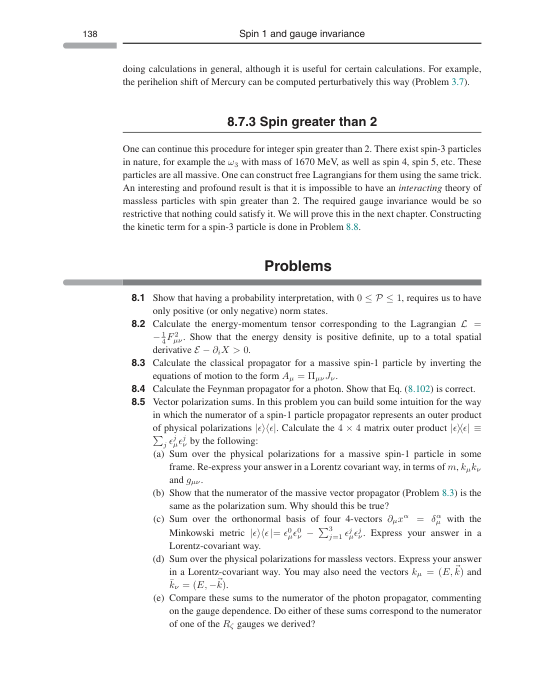
\includegraphics{./figs/8_Spin_1_and_gauge_invariance_page_158.png}

---

